\chapter{Spielidee}

Basierend auf der vorgestellten Engine wurde im Verlauf des Projekts ein eigenes kleines Puzzle-Spiel mit dem Namen ''Troubled Souls'' entwickelt. Dabei handelt es sich um eine abgewandelte Variante einer von Christoph Kapffer im Rahmen des Master-Projekts ''Quantum Quest'' entwickelten Spielidee namens \textbf{\href{http://wiki.htw-berlin.de/display/IMIM/Sammlung+von+Spielkonzepten\#SammlungvonSpielkonzepten-14.\%22CursorFans\%22}{Cursor Fans}}\footnote{siehe \url{http://wiki.htw-berlin.de/display/IMIM/Sammlung+von+Spielkonzepten\#SammlungvonSpielkonzepten-14.\%22CursorFans\%22}}.

\begin{figure}[h] % h = here
	\centering
		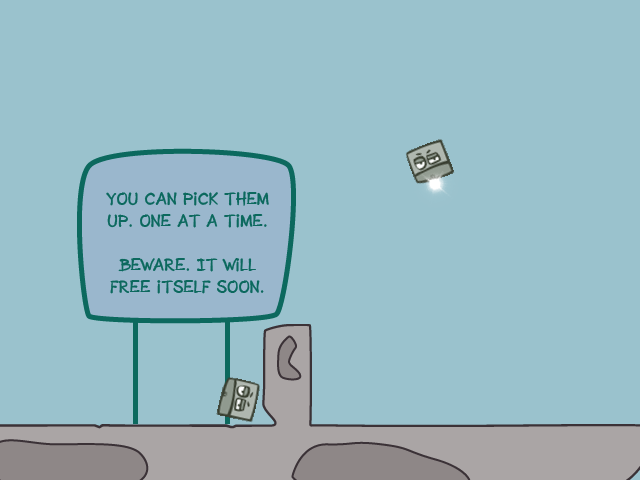
\includegraphics[scale=0.6]{images/screenshot_game.png}
	\caption{Screenshot aus ''Troubled Souls''}
\end{figure}

Ziel in ''Troubled Souls'' ist es eine Schar von \textit{verirrten Seelen} an Hindernissen und Gefahren vorbei sicher an das Ende des Levels zu führen. Diese Seelen folgen vehement der \textit{Quelle des Lebens} - einem mysteriösem Licht, welches an den Mouse-Cursor des Spielers gebunden ist. Sie werden von diesem Licht magisch angezogen und bewegen sich ununterbrochen in dessen Richtung, selbst wenn es ihren eigenen Tod, beispielsweise durch den Sturz in den Abgrund, bedeutet. Sie können nicht anders, denn sollte sich die Quelle des Lebens zu weit von ihnen entfernen, sterben sie ebenfalls.

Aufgabe des Spielers ist es also die Seelen durch die Bewegung der Mouse in die richtige Richtung zu führen. Dabei kann er eine einzelne Seele auch für einige Sekunden hochheben und über Abgründe hiefen. Dabei muss er jedoch darauf achten, dass die anderen dabei nicht in ihr Verderben laufen. Und auch die eine Seele, die er trägt, wird sich nach kurzer Zeit losreißen. 

Um sein Ziel zu erreichen, muss der Spieler die Seelen also geschickt von einander separieren und gleichzeitig darauf achten, sie nicht zu weit voneinander (und somit auch von der Quelle) zu entfernen. Dafür steht ihm aktuell auch ein weiterer Gegenstand, der sogenannte Blocker, zur Verfügung. Dabei handelt es sich um ein physikalisches Hindernis, welches der Spieler selbst bewegen und clever positionieren muss.

\chapter{Aufbau}

Das Spiel selbst ist eine erweiterte Instanz von \textprog{BaseGame}. Innerhalb dieser Instanz werden die \textprog{InputActions} festgelegt, welche für die Steuerung des Spiels sorgen. Zusätzlich implementiert es eine \textprog{update}-Methode, welche die unterschiedlichen Manager sowie das Level aktualisiert und sich um die Bewegung der Kamera kümmert.

\section{Spielobjekte}

Die Hauptspielobjekte sind einfache Boxen, die Troubled Souls, die Quelle des Lebens, Todes-Zonen sowie Blocker. Daneben gibt es noch individuelle Spielobjekte, die zum Gameplay des Levels gehören.

Die Spielobjekte existieren alle in einem eigenen Modul, welches für gewöhnlich eine \textprog{create}-Funktion bereitstellt. Innerhalb dieser Funktion wird eine Instanz von \textprog{BaseGameObject} erstellt und die notwendigen Plugins (und teils Konfigurationen) hinzugefügt.

\subsection{Boxen}

Um die Erstellung des Levels zu vereinfachen gibt es das Modul \textprog{BoxWithPhysics}, mit welchem man einfach über die Angabe von Position und Größe ein Box-Spielobjekt erstellen kann. Wenn gewünscht kann man bei der Erstellung auch Farbe, Textur oder spezielle physikalische Eigenschaften übergeben.

\subsection{Troubled Souls}

Troubled Souls sind im Modul \textprog{DarkSoul} implementiert. In dessen \textprog{create}-Funktion wird eine einfaches Spielobjekt mit textureller Grafik und Physik erstellt und als dynamisches Physikobjekt deklariert. Die Spiellogik wird diesem Object durch das in derselben Datei vorzufindende \textprog{Plugin\_LogicDarkSoul} hinzugefügt. Alle Spielobjekte mit eigenem Gameplay verfügen über ein eigenes Logik-Plugin. Die Möglichkeit eine verirrte Seele aufzunehmen wird dem Spielobjekt durch das \textprog{Plugin\_Pickable} hinzugefügt.

Innerhalb der Logik der Seele wird die Entfernung zum Licht überprüft und sofern diese zu groß ist, startet ein Timer und nach einer kurzen Zeit wird - sofern das Licht nicht wieder näher kommt -  die Seele als tot markiert und der ''Game Over''-Bildschirm angezeigt.

Die Logik steuert zudem die Bewegung der Seelen. Diese bewegen sich physikalisch gesteuert in x-Richtung des Lichts und beginnen zu springen, sobald sie in einer gewissen Nähe sind. Dabei gibt es eine Maximal-Geschwindigkeit, welche über Physik-Impulse gesteuert wird. Die Bewegung wird ausgeschaltet, sobald die Seele hochgenommen wird. Nach einigen Sekunden lässt sie sich allerdings von selbst fallen und der Bewegungs-Algorithmus setzt wieder ein. Wird eine Seele fallen gelassen bzw. reißt sie sich selbst los, so wird ihre Geschwindigkeit gekappt, sodass sie schlicht runterfällt, da man sie ansonsten einfach durch das Level werfen könnte.

Das Plugin fängt zusätzlich die Kollisionen des Physik-Objektes ab. Kollidiert es mit einem als ''DeathZone'' markierten Objekt, so wird die Seele als tot markiert.

\subsection{Quelle des Lebens}

Die Quelle des Lebens ist im Modul \textprog{Cursor} definiert. Ebenso wie die Seelen besitzt sie ein eigenes Logik-Plugin. Das Licht folgt grob dem Cursor, hat dabei allerdings eine Maximalgeschwindigkeit. Erreicht es die Nähe des Cursors, so fliegt es zufällig in dessen unmittelbarer Umgebung umher. Gleichzeitig ändert es seine Farbe abhängig von der Entfernung zur entferntesten Seele um dem Spieler einen Indikator zu geben, ob der Cursor gefährlich weit weg ist.

Das Licht nutzt zur Darstellung das \textprog{Plugin\_SimpleGraphicsTexture2D}. Allerdings wird der Shader bei Initialisierung der Logik durch eine leicht abgewandelte Version des Fragment-Shaders ausgetauscht um die Farbveränderung zu ermöglichen.

\subsection{Blocker}

Ein Blocker-Spielobjekt hat eine spezielle Physik. Es muss dynamisch sein, sodass der Spieler es hochheben und werfen kann, gleichzeitig muss für die Troubled Souls statisch (mit unendlicher Masse) sein, sodass diese den Blocker nicht bewegen können.

Dies wird dadurch realisiert, dass der Blocker aus zwei physikalischen Objekten besteht. Einem dynamischen, welches so eingestellt ist, dass es nicht mit den Seelen kollidiert (sprich hindurchfliegen würde) und ein statisches, welches mit den Seelen kollidiert. Durch das Logik-Plugin werden Position und Rotation des statischen Körpers auf die Werte des dynamischen Körpers gesetzt, sodass dieses sich exakt mit dem dynamischen Körper mitbewegt ohne von den Physikkörpern der Seelen abgelenkt werden zu können.

\section{Level}

Aktuell ist ein Level implementiert, welches in seiner \textprog{create}-Funktion alle Spielobjekte erzeugt und positioniert.

Neben den bereits beschriebenen Spielobjekten enthält es zusätzlich zwei weitere dynamische Objekte: einen fallenden Block sowie einen sich auf und ab bewegenden Block. Beide sind in der Lage die Seelen zu zerquetschen und somit zu töten.

Damit die Seelen nur sterben, wenn sie die Unterseite der Blöcke bewegen, sind diese aus zwei Einzelteilen aufgebaut: einem dynamischen Körper sowie einem Sensor, der etwas kleiner und nach unten verschoben ist und sich mit dem dynamischen Körper mitbewegt. Berührt eine Seele den Sensor, so stirbt sie.

Damit die Physik nicht anfängt zu spinnen, sobald der Block von oben auf eine Seele fällt, sind die Blöcke von unten durchlässig, sprich Kollisionen werden ignoriert. Dies geschieht, indem man den den Kollisions-Kontakt innerhalb der \textprog{onPreSolve}-Methode (siehe Physik-Teil) ignoriert.

\newpage
\section{Menu}

Die GUI des Menüs für das Spiel wird nicht - wie man es erwarten könnte - durch WebGL gerendert, sondern durch HTML-Elemente dargestellt, welche über dem Viewport des Spiels positioniert sind. Die entsprechenden Elemente sind im HTML-Code enthalten und werden vom Javascript-Code des Spiels ein- und ausgeblendet. Die Verwendung von HTML hat den Vorteil, dass kein eigenes GUI-System innerhalb der Engine entwickelt werden musste.

\begin{figure}[h] % h = here
	\centering
		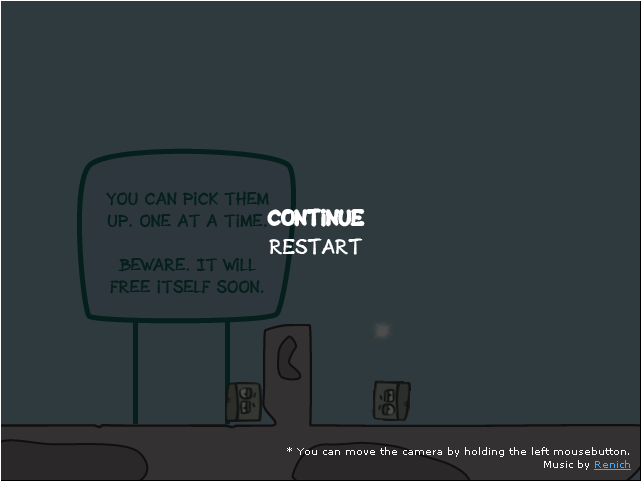
\includegraphics[scale=0.6]{images/screenshot_ui.png}
	\caption{Screenshot des User-Interfaces von ''Troubled Souls''}
\end{figure}

